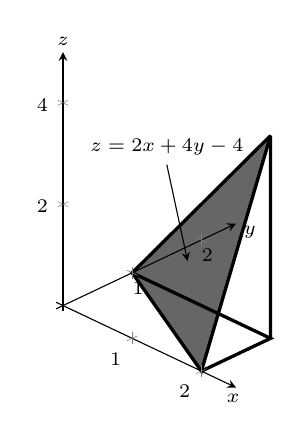
\begin{tikzpicture}[>=stealth]
\begin{axis}%
[width=175pt,height=200pt,
tick label style={font=\scriptsize},axis on top,
			axis lines=center,
			view={45}{25},
			name=myplot,
			xtick={1,2},
			ytick={1,2},
			ztick={2,4},
			%extra x ticks={1},
			%minor x tick num=1,
			%minor y tick num=4,
			%minor z tick num=1,
			%extra x tick labels={$a$},
			%extra y ticks={1},
			%extra y tick labels={$a$},
			%extra z ticks={1},
			%extra z tick labels={$h$},
			ymin=-.1,ymax=2.5,
			xmin=-.1,xmax=2.5,
			zmin=-.1, zmax=5,
			every axis x label/.style={at={(axis cs:\pgfkeysvalueof{/pgfplots/xmax},0,0)},xshift=-1pt,yshift=-4pt},
				xlabel={\scriptsize $x$},
			every axis y label/.style={at={(axis cs:0,\pgfkeysvalueof{/pgfplots/ymax},0)},xshift=5pt,yshift=-3pt},
				ylabel={\scriptsize $y$},
				every axis z label/.style={at={(axis cs:0,0,\pgfkeysvalueof{/pgfplots/zmax})},xshift=0pt,yshift=4pt},
				zlabel={\scriptsize $z$}
			]

%\addplot3[domain=-2:0,y domain=-2:0,%surf, %fill=white,
%%colormap={mp2}{\colormaptwo},opacity=.6,faceted color=black!40,
%samples=10,%samples y=10, very thin
%{\colortwo},very thick,samples y=0,smooth] ({0},{x},{x^2/2});
%
%\addplot3[domain=-2:0,y domain=-2:0,%surf, %fill=white,
%%colormap={mp2}{\colormaptwo},opacity=.6,faceted color=black!40,
%samples=10,%samples y=10, very thin
%{\colortwo},very thick,samples y=0,smooth] ({2},{x},{x^2/2});

%\addplot3[domain=0:3,y domain=0:9,surf, %fill=white,
%colormap={mp2}{\colormaptwo},opacity=.6,faceted color=black!40,samples=21,samples y=21, very thin] ({x},{y},{sqrt(y^2-9*x^2)});


%\addplot3[domain=0:90,y domain=0:9,surf, %fill=white,
%colormap={mp2}{\colormapplaneone},opacity=.6,faceted color=black!40,samples=11,samples y=11, very thin] ({y*cos(x)/3},{y},{y*sin(x)});

\draw [{\colorone}, very thick] (axis cs: 0,1,0) -- (axis cs: 2,1,0) -- (axis cs: 2,0,0) 
																(axis cs: 2,1,0) -- (axis cs: 2,1,4);
																
																

%\addplot3[domain=0:90,y domain=-2:0,%surf, %fill=white,
%%colormap={mp2}{\colormaptwo},opacity=.6,faceted color=black!40,
%samples=10,%samples y=10, very thin
%{\colorone},very thick,samples y=0,smooth] ({9*cos(x)/3},{9},{9*sin(x)}) -- (axis cs: 0,0,0);

%\draw [{\colorone}, very thick] (axis cs: 3,0,0) -- (axis cs: 1,0,0) -- (axis cs: 1,0,1)
																%(axis cs: 3,2,0) -- (axis cs: 1,2,0) -- (axis cs: 1,2,1)
																%(axis cs: 1,0,0) --  (axis cs: 1,2,0);
%
%
\draw [{\coloronefill}, very thin,fill={\coloronefill},opacity=.6] (axis cs: 0,1,0) -- (axis cs: 2,0,0) -- (axis cs: 2,1,4) --  cycle;
%%
\draw [{\colorone}, very thick] (axis cs: 2,1,4) -- (axis cs: 0,1,0) -- (axis cs: 2,0,0) -- (axis cs: 2,1,4) ;
%%
\draw [->] (axis cs: 1.5,0,3.75) node [above] {\scriptsize $z= 2x+4y-4$} -- (axis cs: .8,1,.75);
%
%\draw  (axis cs: 2,-1.2,.7) node [below,rotate=-65] {\scriptsize $z= \frac12y^2$};% -- (axis cs: 1,0,.5);




\end{axis}


\end{tikzpicture}












